\documentclass{beamer}
\title[$E_r$-Generating Terms in L-H Transitions]{Radial Electric Field-Generating Terms in L-H Transitions}
\author[K.A. Blondino]{
\includegraphics[height=1cm]{../../Graphics/tue_fusion_logo.png} \\ Kevin A. Blondino \\
	Supervisor: dr. H.J. de Blank, TU/e \& DIFFER}
\institute[TU/e]{Eindhoven University of Technology \\
	\medskip
	\textit{k.blondino@student.tue.nl}}
\date{14 August 2017}

%{{{ Presentation Style and Color
\mode<presentation>
{
%\usetheme{default}
%\usetheme{AnnArbor}
%\usetheme{Antibes}
%\usetheme{Bergen}
%\usetheme{Berkeley}
%\usetheme{Berlin}
%\usetheme{Boadilla}
%\usetheme{CambridgeUS}
%\usetheme{Copenhagen}
%\usetheme{Darmstadt}
%\usetheme{Dresden}
%\usetheme{Frankfurt}
%\usetheme{Goettingen}
%\usetheme{Hannover}
%\usetheme{Ilmenau}
%\usetheme{JuanLesPins}
%\usetheme{Luebeck}
%\usetheme{Madrid}
%\usetheme{Malmoe}
%\usetheme{Marburg}
%\usetheme{Montpellier}
%\usetheme{PaloAlto}
%\usetheme{Pittsburgh}
%\usetheme{Rochester}
%\usetheme{Singapore}
\usetheme{Szeged}
%\usetheme{Warsaw}

%\usecolortheme{albatross}
\usecolortheme{beaver}
%\usecolortheme{beetle}
%\usecolortheme{crane}
%\usecolortheme{dolphin}
%\usecolortheme{dove}
%\usecolortheme{fly}
%\usecolortheme{lily}
%\usecolortheme{orchid}
%\usecolortheme{rose}
%\usecolortheme{seagull}
%\usecolortheme{seahorse}
%\usecolortheme{whale}
%\usecolortheme{wolverine}

%\setbeamertemplate{caption}[numbered]
\setbeamertemplate{bibliography item}{\insertbiblabel}
%\setbeamertemplate{footline} % To remove the footer line in all slides uncomment this line
%\setbeamertemplate{footline}[page number] % To replace the footer line in all slides with a simple slide count uncomment this line

%\setbeamertemplate{navigation symbols}{} % To remove the navigation symbols from the bottom of all slides uncomment this line
}
%}}}

%{{{ Packages
\usepackage{amsmath,graphicx,booktabs,moresize,textpos}
\usepackage[utf8]{inputenc}
\usepackage{caption}
\captionsetup{font=scriptsize,labelfont=bf}
\usepackage[UKenglish]{isodate}
\cleanlookdateon
%}}}

%{{{ Setup References
\usepackage[backend=biber,style=authoryear]{biblatex}
\addbibresource{../../References/References.bib}
\renewcommand*{\nameyeardelim}{\addcomma\addspace}
%}}}

%{{{ Two Figures Side-by-Side
\newsavebox\IBoxA \newsavebox\IBoxB \newlength\IHeight
\newcommand\TwoFig[6]{% Image1 Caption1 Label1 Im2 Cap2 Lab2
	\sbox\IBoxA{\includegraphics[width=0.45\textwidth]{#1}}
	\sbox\IBoxB{\includegraphics[width=0.45\textwidth]{#4}}%
	\ifdim\ht\IBoxA>\ht\IBoxB
		\setlength\IHeight{\ht\IBoxB}%
	\else\setlength\IHeight{\ht\IBoxA}\fi
	\begin{figure}[ht]
		\minipage[t]{0.49\textwidth}\centering
			\includegraphics[height=\IHeight]{#1}
			\caption{#2}\label{#3}
		\endminipage\hfill
		\minipage[t]{0.49\textwidth}\centering
			\includegraphics[height=\IHeight]{#4}
			\caption{#5}\label{#6}
		\endminipage
	\end{figure}%
}
%}}}

\begin{document}
% Title page
\begin{frame}
\titlepage
\end{frame}

\addtobeamertemplate{frametitle}{}
{
\begin{textblock*}{100mm}(0.85\textwidth,-1cm)
	
\includegraphics[height=1cm,width=2cm]{../../Graphics/tue_fusion_logo.png}
\end{textblock*}
}

%--------------------------------------
% Overview
\begin{frame}
\frametitle{Overview}
\tableofcontents
\end{frame}

%--------------------------------------

\section{Background}
%\subsection{H-mode}
\begin{frame}
\frametitle{H-mode}
\begin{itemize}
	\item In 1982 at ASDEX, H-mode was discovered when heating was increased, which increased confinement time by a factor of around 2 \parencite{wagner_development_1984}.
	\item Anomalous transport has been found to be the dominant transport of particles and energy \parencite{freidberg_plasma_2007}.
	\item H-mode forms as a response to significant reduction in this anomalous transport at the plasma edge.
	\begin{itemize}
		\item The prevailing hypothesis is that high auxiliary power develops strong sheared plasma flow.
		\item It is characterized by its pressure profile that is significantly raised compared to L-mode, and is said to sit on a `pedestal.'
		\item Accordingly, there is a steep gradient at the edge, creating a transport barrier.
	\end{itemize}
\end{itemize}
\end{frame}

\begin{frame}
\frametitle{H-mode}
\begin{figure}
	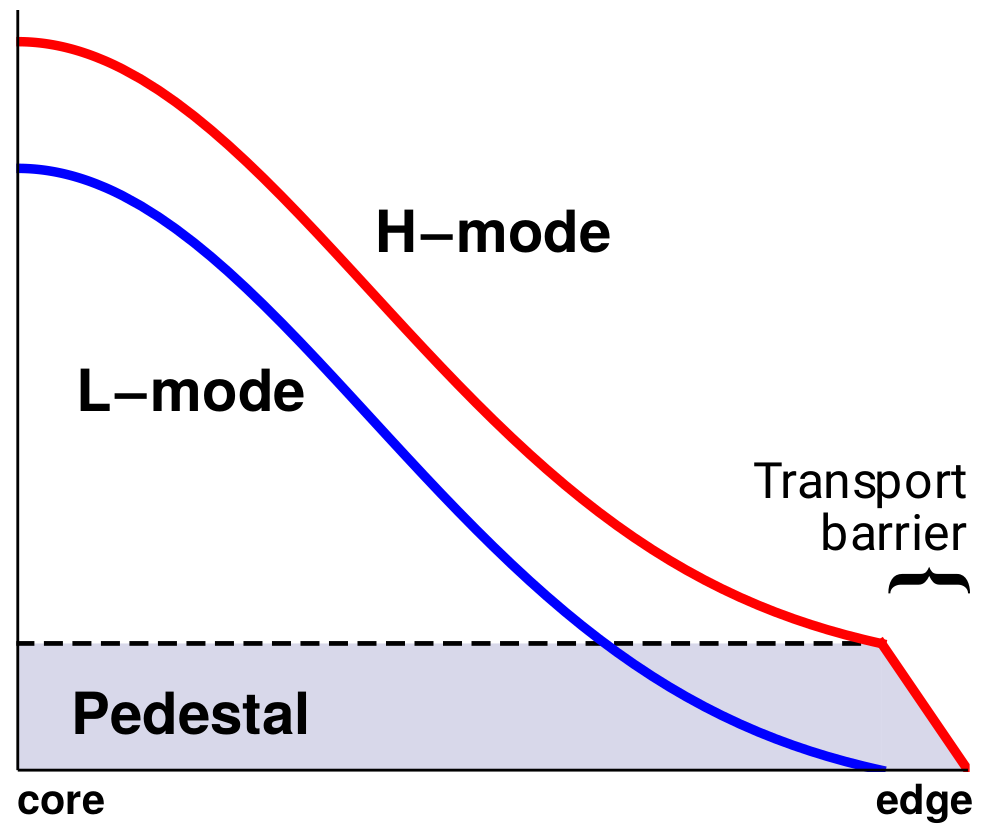
\includegraphics[width=0.5\linewidth]{../../Graphics/L-mode_H-mode_compare.png}
	\caption{A comparison of the radial pressure profiles of L-mode and H-mode.
	The profile of H-mode can be thought of as on a ‘pedestal,’ in which the pressure profile is increase in the core.
	This is due to the transport barrier that is formed at the
	edge \parencite{weymiens_bifurcation_2014}.}
	\label{fig:L-mode_H-mode_compare}
\end{figure}
\end{frame}

%--------------------------------------

%\subsection{Transition}
\begin{frame}
\frametitle{Transition}
\begin{itemize}
	\item The L-H transition is a bifurcation in the turbulent transport at the plasma edge.
	\item The cusp bifurcation organizes two different transition dynamics: smooth and sharp.
	\begin{itemize}
		\item The smooth transition occurs for lower density plasmas.
		\item The sharp transition is more common, and exhibits hysteresis.
	\end{itemize}
	\item There is a third type of transition in which the plasma will oscillate between the two modes.
	\begin{itemize}
		\item It occurs when there are no stable states surrounding the cusp bifurcation.
		Mathematically, its existence is dicated by a coupling parameter above a critical value.
	\end{itemize}
\end{itemize}
\end{frame}

\begin{frame}
\frametitle{Transition}
\TwoFig{../../Graphics/Bif_3D.png}
	{Two codimension 1 fold bifurcations, with the parameter $b$ dictating the size of the hysteresis, until the bifurcations merge into a cusp \parencite{weymiens_bifurcation_2014}.}
	{fig:Bif_3D}
	{../../Graphics/3_transitions_single_simple.png}
	{Codimension 3 parameter space with the black line indicating the fold bifurcation. The parameter $b$ dictates the type of transition, including the size of the hysteresis in the sharp transition \parencite{weymiens_bifurcation_2014}.}
	{fig:Bif_types}
\end{frame}

%--------------------------------------

%\subsection{Electric Field}
\begin{frame}
\frametitle{Electric Field}
\begin{equation*}
	E_r \,=\, -\frac{1}{n_j e_j} \frac{\text{d}p_j}{\text{d}r} + V_{\theta j} B_\phi - V_{\phi j} B_\theta
	\label{eq:E_r}
\end{equation*}
\begin{itemize}
	\item The combination of the electric field with the magnetic field creates $\mathbf{E}\times\mathbf{B}$ flows and flow shear, which tears apart eddies.
	\item Changes in the field are associated with changes in the pressure gradient or in plasma poloidal or toroidal flow.
	\begin{itemize}
		\item However, accurately measuring plasma flow velocities and the pressure gradient is very difficult.
		\item Instead, utilize knowledge of the particle fluxes; nonambipolar fluxes generate current.
	\end{itemize}
\end{itemize}
\end{frame}

%\subsection{Nonambipolar Fluxes}
\begin{frame}
\frametitle{Nonambipolar Fluxes}
A few examples:
\begin{itemize}
	\item Charge exchange friction
	\begin{itemize}
		\item There is a loss of ion momentum due to the charge exchange rate that dominates over ionization impact \parencite{toda_condensed_neutrals_1997}.
	\end{itemize}
	\item Ion orbit loss
	\begin{itemize}
		\item Ions that have gyro-orbits or banana orbits that extend outside of the last closed flux surface. The fraction of these that are collisionless is a nonambipolar flux \parencite{chankin_loss_1993}.
	\end{itemize}
	\item Reynolds stress
	\begin{itemize}
		\item Turbulent fluctuations cause perturbations to the flow. For coherent and spatially-varying fluctuations, a nonzero Reynolds stress accelerates poloidal flow \parencite{diamond_poloidal_1991}.
	\end{itemize}
\item Poloidal flux transients, Maxwell stress, magnetic perturbations, etc \parencite{staps_backstepping_2017}.
\end{itemize}
\end{frame}
%}}}

%--------------------------------------

\section{Transition Model}
\begin{frame}
\frametitle{Transition Model}
	The basic model for the transition, developed first by \textcite{itoh_edge_1991}, expanded by \textcite{zohm_dynamic_1994}, and then into the following form by \textcite{weymiens_bifurcation_2014}.
It contains the continuity equations of energy and density to describe H-mode.
\begin{equation*}
	\epsilon\,\frac{\partial Z}{\partial t} \,=\, \mu\,\frac{\partial^2 Z}{\partial x^2} + \frac{c_n T}{n^2} \frac{\partial n}{\partial x} + \frac{c_T}{n} \frac{\partial T}{\partial x} + G(Z)
	\label{eq:pde}
\end{equation*}
This model uses $Z$, the radial electric field normalized with respect to the ion Larmor (gyro-)radius $\rho_{\theta i}$ and temperature $T = T_i = T_e$.
\begin{equation*}
	Z \,=\, \frac{\rho_{\theta i} \, e \, E_r}{T}, ~~~~~ \rho_{\theta i} \,=\, \frac{m_i \, v_{\phi i}}{e B_\theta}
	\label{eq:normalization}
\end{equation*}
\end{frame}

\begin{frame}
\frametitle{Transition Model}
\begin{equation*}
	\epsilon\,\frac{\partial Z}{\partial t} \,=\, \mu\,\frac{\partial^2 Z}{\partial x^2} + \frac{c_n T}{n^2} \frac{\partial n}{\partial x} + \frac{c_T}{n} \frac{\partial T}{\partial x} + G(Z)
	%\label{eq:pde}
\end{equation*}
	\begin{itemize}
		\item The LHS represents the radial current due to polarization.
		\begin{itemize}
			\item $\epsilon \,\equiv\, \dfrac{B_\theta^2}{B^2 \nu_i}$ is the dielectric constant.
			Dictates timescale, with smaller values corresponding to sharper temporal transitions.
		\end{itemize}
		\item The 2nd derivative term describes the radial current due to the anomalous shear viscosity of the $\mathbf{E}\times\mathbf{B}$ drift.
		\begin{itemize}
			\item $\mu$ is the ratio of viscosity to collision frequency. Smaller values result in sharper spatial transitions.
		\end{itemize}
	\end{itemize}
\end{frame}

\begin{frame}
\frametitle{Transition Model}
\begin{equation*}
	\epsilon\,\frac{\partial Z}{\partial t} \,=\, \mu\,\frac{\partial^2 Z}{\partial x^2} + \frac{c_n T}{n^2} \frac{\partial n}{\partial x} + \frac{c_T}{n} \frac{\partial T}{\partial x} + G(Z)
	%\label{eq:pde}
\end{equation*}
	\begin{itemize}
		\item The spatial 1st derivatives are an accumulation of all 1st derivative terms from the remaining fluxes.
		\item $G(Z)$ is a cubic polynomial that approximates the remaining non-derivative terms of the fluxes.
		\begin{equation*}
			G(Z) \,=\, a + b(Z - Z_S) + c(Z - Z_S)^3
			\label{eq:G_func}
		\end{equation*}
		\begin{itemize}
			\item The coefficients $c_T$, $c_n$, and in $G$ are determined by the summation of all the relevant processes.
		\end{itemize}
	\end{itemize}
\end{frame}
%}}}

%--------------------------------------

\section{Research Plan}
\begin{frame}
\frametitle{Current State and Central Question}
\begin{itemize}
	\item Because H-mode is essentially necessary for fusion in tokamaks, comprehensive knowledge of its formation is needed to predict and control.
	\item Substantial investigation has been done in identifying processes to generate the field \parencite{connor_review_2000}.
	\begin{itemize}
		\item However, none have investigated comprehensively without the use of some form of scaling laws.
	\end{itemize}
\end{itemize}
\vfill
\fbox{
	\parbox{\textwidth}{
	\textbf{Which electric field-generating terms are dominant in concrete tokamak experiments?}
	}}
\end{frame}

\begin{frame}
\frametitle{Research Plan}
Specifically, the parameters of ASDEX-U will be used in the transition model.
\begin{itemize}
	\item Which nonambipolar fluxes should be considered for investigation?
	\begin{itemize}
		\item Some are negligible, such as magnetic ripple loss.
	\end{itemize}
	\item Identify the ideal form and relative strengths of each flux.
	\begin{itemize}
		\item Since the model is nonlinear, it is potentially highly sensitive to relative strengths.
	\end{itemize}
	\item Previous investigations were somewhat limited in input power \parencite{staps_backstepping_2017}. Expanding the regime could make the study more comprehensive.
	\item Time permitting, determine how each term theoretically scales with machine size and what that implies for extrapolation.
\end{itemize}
\end{frame}

%--------------------------------------

%\section{References}
\begin{frame}
\frametitle{References}
\renewcommand*{\bibfont}{\tiny}
%\nocite{*}
\printbibliography
\end{frame}
%}}}

\end{document}

